\documentclass[1p]{elsarticle_modified}
%\bibliographystyle{elsarticle-num}

%\usepackage[colorlinks]{hyperref}
%\usepackage{abbrmath_seonhwa} %\Abb, \Ascr, \Acal ,\Abf, \Afrak
\usepackage{amsfonts}
\usepackage{amssymb}
\usepackage{amsmath}
\usepackage{amsthm}
\usepackage{scalefnt}
\usepackage{amsbsy}
\usepackage{kotex}
\usepackage{caption}
\usepackage{subfig}
\usepackage{color}
\usepackage{graphicx}
\usepackage{xcolor} %% white, black, red, green, blue, cyan, magenta, yellow
\usepackage{float}
\usepackage{setspace}
\usepackage{hyperref}

\usepackage{tikz}
\usetikzlibrary{arrows}

\usepackage{multirow}
\usepackage{array} % fixed length table
\usepackage{hhline}

%%%%%%%%%%%%%%%%%%%%%
\makeatletter
\renewcommand*\env@matrix[1][\arraystretch]{%
	\edef\arraystretch{#1}%
	\hskip -\arraycolsep
	\let\@ifnextchar\new@ifnextchar
	\array{*\c@MaxMatrixCols c}}
\makeatother %https://tex.stackexchange.com/questions/14071/how-can-i-increase-the-line-spacing-in-a-matrix
%%%%%%%%%%%%%%%

\usepackage[normalem]{ulem}

\newcommand{\msout}[1]{\ifmmode\text{\sout{\ensuremath{#1}}}\else\sout{#1}\fi}
%SOURCE: \msout is \stkout macro in https://tex.stackexchange.com/questions/20609/strikeout-in-math-mode

\newcommand{\cancel}[1]{
	\ifmmode
	{\color{red}\msout{#1}}
	\else
	{\color{red}\sout{#1}}
	\fi
}

\newcommand{\add}[1]{
	{\color{blue}\uwave{#1}}
}

\newcommand{\replace}[2]{
	\ifmmode
	{\color{red}\msout{#1}}{\color{blue}\uwave{#2}}
	\else
	{\color{red}\sout{#1}}{\color{blue}\uwave{#2}}
	\fi
}

\newcommand{\Sol}{\mathcal{S}} %segment
\newcommand{\D}{D} %diagram
\newcommand{\A}{\mathcal{A}} %arc


%%%%%%%%%%%%%%%%%%%%%%%%%%%%%5 test

\def\sl{\operatorname{\textup{SL}}(2,\Cbb)}
\def\psl{\operatorname{\textup{PSL}}(2,\Cbb)}
\def\quan{\mkern 1mu \triangleright \mkern 1mu}

\theoremstyle{definition}
\newtheorem{thm}{Theorem}[section]
\newtheorem{prop}[thm]{Proposition}
\newtheorem{lem}[thm]{Lemma}
\newtheorem{ques}[thm]{Question}
\newtheorem{cor}[thm]{Corollary}
\newtheorem{defn}[thm]{Definition}
\newtheorem{exam}[thm]{Example}
\newtheorem{rmk}[thm]{Remark}
\newtheorem{alg}[thm]{Algorithm}

\newcommand{\I}{\sqrt{-1}}
\begin{document}

%\begin{frontmatter}
%
%\title{Boundary parabolic representations of knots up to 8 crossings}
%
%%% Group authors per affiliation:
%\author{Yunhi Cho} 
%\address{Department of Mathematics, University of Seoul, Seoul, Korea}
%\ead{yhcho@uos.ac.kr}
%
%
%\author{Seonhwa Kim} %\fnref{s_kim}}
%\address{Center for Geometry and Physics, Institute for Basic Science, Pohang, 37673, Korea}
%\ead{ryeona17@ibs.re.kr}
%
%\author{Hyuk Kim}
%\address{Department of Mathematical Sciences, Seoul National University, Seoul 08826, Korea}
%\ead{hyukkim@snu.ac.kr}
%
%\author{Seokbeom Yoon}
%\address{Department of Mathematical Sciences, Seoul National University, Seoul, 08826,  Korea}
%\ead{sbyoon15@snu.ac.kr}
%
%\begin{abstract}
%We find all boundary parabolic representation of knots up to 8 crossings.
%
%\end{abstract}
%\begin{keyword}
%    \MSC[2010] 57M25 
%\end{keyword}
%
%\end{frontmatter}

%\linenumbers
%\tableofcontents
%
\newcommand\colored[1]{\textcolor{white}{\rule[-0.35ex]{0.8em}{1.4ex}}\kern-0.8em\color{red} #1}%
%\newcommand\colored[1]{\textcolor{white}{ #1}\kern-2.17ex	\textcolor{white}{ #1}\kern-1.81ex	\textcolor{white}{ #1}\kern-2.15ex\color{red}#1	}

{\Large $\underline{12n_{0610}~(K12n_{0610})}$}

\setlength{\tabcolsep}{10pt}
\renewcommand{\arraystretch}{1.6}
\vspace{1cm}\begin{tabular}{m{100pt}>{\centering\arraybackslash}m{274pt}}
\multirow{5}{120pt}{
	\centering
	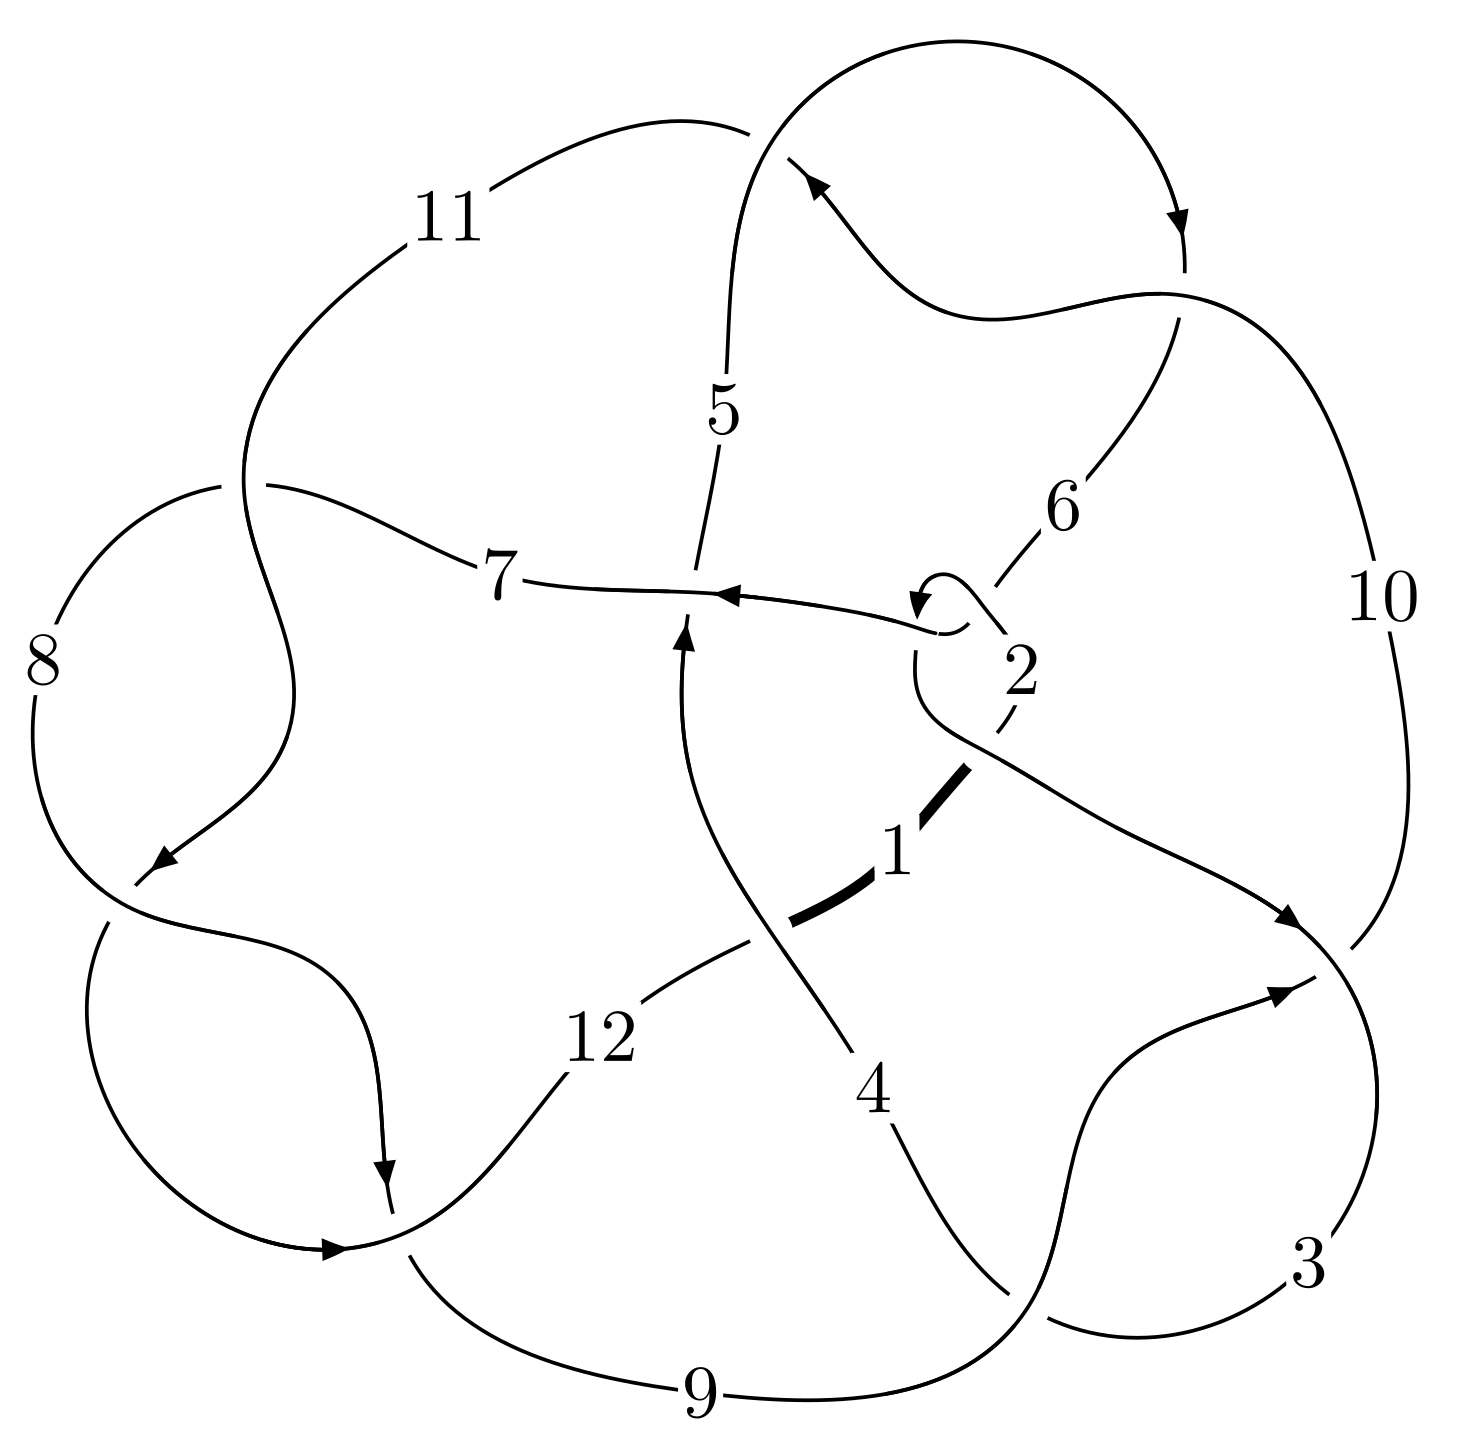
\includegraphics[width=112pt]{../../../GIT/diagram.site/Diagrams/png/2699_12n_0610.png}\\
\ \ \ A knot diagram\footnotemark}&
\allowdisplaybreaks
\textbf{Linearized knot diagam} \\
\cline{2-2}
 &
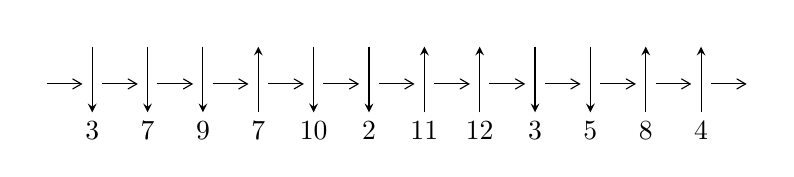
\begin{tikzpicture}[x=20pt, y=17pt]
	% nodes
	\node (C0) at (0, 0) {};
	\node (C1) at (1, 0) {};
	\node (C1U) at (1, +1) {};
	\node (C1D) at (1, -1) {3};

	\node (C2) at (2, 0) {};
	\node (C2U) at (2, +1) {};
	\node (C2D) at (2, -1) {7};

	\node (C3) at (3, 0) {};
	\node (C3U) at (3, +1) {};
	\node (C3D) at (3, -1) {9};

	\node (C4) at (4, 0) {};
	\node (C4U) at (4, +1) {};
	\node (C4D) at (4, -1) {7};

	\node (C5) at (5, 0) {};
	\node (C5U) at (5, +1) {};
	\node (C5D) at (5, -1) {10};

	\node (C6) at (6, 0) {};
	\node (C6U) at (6, +1) {};
	\node (C6D) at (6, -1) {2};

	\node (C7) at (7, 0) {};
	\node (C7U) at (7, +1) {};
	\node (C7D) at (7, -1) {11};

	\node (C8) at (8, 0) {};
	\node (C8U) at (8, +1) {};
	\node (C8D) at (8, -1) {12};

	\node (C9) at (9, 0) {};
	\node (C9U) at (9, +1) {};
	\node (C9D) at (9, -1) {3};

	\node (C10) at (10, 0) {};
	\node (C10U) at (10, +1) {};
	\node (C10D) at (10, -1) {5};

	\node (C11) at (11, 0) {};
	\node (C11U) at (11, +1) {};
	\node (C11D) at (11, -1) {8};

	\node (C12) at (12, 0) {};
	\node (C12U) at (12, +1) {};
	\node (C12D) at (12, -1) {4};
	\node (C13) at (13, 0) {};

	% arrows
	\draw[->,>={angle 60}]
	(C0) edge (C1) (C1) edge (C2) (C2) edge (C3) (C3) edge (C4) (C4) edge (C5) (C5) edge (C6) (C6) edge (C7) (C7) edge (C8) (C8) edge (C9) (C9) edge (C10) (C10) edge (C11) (C11) edge (C12) (C12) edge (C13) ;	\draw[->,>=stealth]
	(C1U) edge (C1D) (C2U) edge (C2D) (C3U) edge (C3D) (C4D) edge (C4U) (C5U) edge (C5D) (C6U) edge (C6D) (C7D) edge (C7U) (C8D) edge (C8U) (C9U) edge (C9D) (C10U) edge (C10D) (C11D) edge (C11U) (C12D) edge (C12U) ;
	\end{tikzpicture} \\
\hhline{~~} \\& 
\textbf{Solving Sequence} \\ \cline{2-2} 
 &
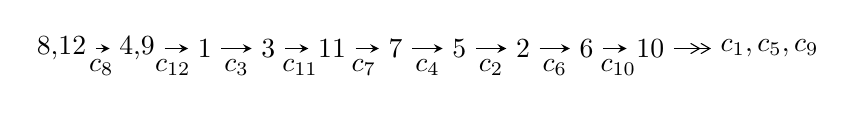
\begin{tikzpicture}[x=23pt, y=7pt]
	% node
	\node (A0) at (-1/8, 0) {8,12};
	\node (A1) at (17/16, 0) {4,9};
	\node (A2) at (17/8, 0) {1};
	\node (A3) at (25/8, 0) {3};
	\node (A4) at (33/8, 0) {11};
	\node (A5) at (41/8, 0) {7};
	\node (A6) at (49/8, 0) {5};
	\node (A7) at (57/8, 0) {2};
	\node (A8) at (65/8, 0) {6};
	\node (A9) at (73/8, 0) {10};
	\node (C1) at (1/2, -1) {$c_{8}$};
	\node (C2) at (13/8, -1) {$c_{12}$};
	\node (C3) at (21/8, -1) {$c_{3}$};
	\node (C4) at (29/8, -1) {$c_{11}$};
	\node (C5) at (37/8, -1) {$c_{7}$};
	\node (C6) at (45/8, -1) {$c_{4}$};
	\node (C7) at (53/8, -1) {$c_{2}$};
	\node (C8) at (61/8, -1) {$c_{6}$};
	\node (C9) at (69/8, -1) {$c_{10}$};
	\node (A10) at (11, 0) {$c_{1},c_{5},c_{9}$};

	% edge
	\draw[->,>=stealth]	
	(A0) edge (A1) (A1) edge (A2) (A2) edge (A3) (A3) edge (A4) (A4) edge (A5) (A5) edge (A6) (A6) edge (A7) (A7) edge (A8) (A8) edge (A9) ;
	\draw[->>,>={angle 60}]	
	(A9) edge (A10);
\end{tikzpicture} \\ 

\end{tabular} \\

\footnotetext{
The image of knot diagram is generated by the software ``\textbf{Draw programme}" developed by Andrew Bartholomew(\url{http://www.layer8.co.uk/maths/draw/index.htm\#Running-draw}), where we modified some parts for our purpose(\url{https://github.com/CATsTAILs/LinksPainter}).
}\phantom \\ \newline 
\centering \textbf{Ideals for irreducible components\footnotemark of $X_{\text{par}}$} 
 
\begin{align*}
I^u_{1}&=\langle 
31 u^{18}+105 u^{17}+\cdots+2 b+78,\;-23 u^{18}-77 u^{17}+\cdots+4 a-56,\;u^{19}+5 u^{18}+\cdots-2 u+4\rangle \\
I^u_{2}&=\langle 
- u^{10}- u^9+5 u^8+5 u^7-7 u^6-7 u^5+2 u^4+2 u^3-2 u^2+b-2 u+1,\\
\phantom{I^u_{2}}&\phantom{= \langle  }2 u^{10}-13 u^8- u^7+29 u^6+6 u^5-25 u^4-11 u^3+9 u^2+a+6 u-5,\\
\phantom{I^u_{2}}&\phantom{= \langle  }u^{11}-7 u^9- u^8+17 u^7+6 u^6-16 u^5-11 u^4+5 u^3+6 u^2-2 u-1\rangle \\
I^u_{3}&=\langle 
22 u^5 a^3-7 u^5 a^2+\cdots+11 a^3-12 a^2,\;2 u^5 a^3-2 u^5 a^2+\cdots-9 a+31,\;u^6- u^5-3 u^4+2 u^3+2 u^2+u-1\rangle \\
\\
\end{align*}
\raggedright * 3 irreducible components of $\dim_{\mathbb{C}}=0$, with total 54 representations.\\
\footnotetext{All coefficients of polynomials are rational numbers. But the coefficients are sometimes approximated in decimal forms when there is not enough margin.}
\newpage
\renewcommand{\arraystretch}{1}
\centering \section*{I. $I^u_{1}= \langle 31 u^{18}+105 u^{17}+\cdots+2 b+78,\;-23 u^{18}-77 u^{17}+\cdots+4 a-56,\;u^{19}+5 u^{18}+\cdots-2 u+4 \rangle$}
\flushleft \textbf{(i) Arc colorings}\\
\begin{tabular}{m{7pt} m{180pt} m{7pt} m{180pt} }
\flushright $a_{8}=$&$\begin{pmatrix}1\\0\end{pmatrix}$ \\
\flushright $a_{12}=$&$\begin{pmatrix}0\\u\end{pmatrix}$ \\
\flushright $a_{4}=$&$\begin{pmatrix}\frac{23}{4} u^{18}+\frac{77}{4} u^{17}+\cdots-\frac{73}{4} u+14\\-\frac{31}{2} u^{18}-\frac{105}{2} u^{17}+\cdots+\frac{89}{2} u-39\end{pmatrix}$ \\
\flushright $a_{9}=$&$\begin{pmatrix}1\\- u^2\end{pmatrix}$ \\
\flushright $a_{1}=$&$\begin{pmatrix}-\frac{5}{2} u^{18}-8 u^{17}+\cdots+7 u-\frac{11}{2}\\\frac{11}{2} u^{18}+\frac{35}{2} u^{17}+\cdots-\frac{23}{2} u+12\end{pmatrix}$ \\
\flushright $a_{3}=$&$\begin{pmatrix}\frac{21}{4} u^{18}+\frac{71}{4} u^{17}+\cdots-\frac{63}{4} u+13\\-\frac{27}{2} u^{18}-\frac{93}{2} u^{17}+\cdots+\frac{81}{2} u-35\end{pmatrix}$ \\
\flushright $a_{11}=$&$\begin{pmatrix}- u\\u\end{pmatrix}$ \\
\flushright $a_{7}=$&$\begin{pmatrix}- u^2+1\\u^2\end{pmatrix}$ \\
\flushright $a_{5}=$&$\begin{pmatrix}-\frac{35}{4} u^{18}-\frac{121}{4} u^{17}+\cdots+\frac{97}{4} u-23\\\frac{17}{2} u^{18}+\frac{59}{2} u^{17}+\cdots-\frac{47}{2} u+21\end{pmatrix}$ \\
\flushright $a_{2}=$&$\begin{pmatrix}\frac{7}{4} u^{18}+\frac{17}{4} u^{17}+\cdots-\frac{9}{4} u^2+\frac{11}{4} u\\-\frac{9}{2} u^{18}-\frac{25}{2} u^{17}+\cdots+\frac{9}{2} u-7\end{pmatrix}$ \\
\flushright $a_{6}=$&$\begin{pmatrix}\frac{17}{2} u^{18}+28 u^{17}+\cdots-18 u+\frac{39}{2}\\-\frac{19}{2} u^{18}-\frac{61}{2} u^{17}+\cdots+\frac{39}{2} u-20\end{pmatrix}$ \\
\flushright $a_{10}=$&$\begin{pmatrix}2 u^{18}+\frac{15}{2} u^{17}+\cdots-\frac{15}{2} u+\frac{13}{2}\\-\frac{5}{2} u^{18}-\frac{19}{2} u^{17}+\cdots+\frac{21}{2} u-8\end{pmatrix}$\\&\end{tabular}
\flushleft \textbf{(ii) Obstruction class $= -1$}\\~\\
\flushleft \textbf{(iii) Cusp Shapes $= 3 u^{18}+13 u^{17}-4 u^{16}-78 u^{15}-41 u^{14}+166 u^{13}+76 u^{12}-219 u^{11}+32 u^{10}+271 u^9-88 u^8-117 u^7+158 u^6+35 u^5-79 u^4+21 u^3+27 u^2-14 u+2$}\\~\\
\newpage\renewcommand{\arraystretch}{1}
\flushleft \textbf{(iv) u-Polynomials at the component}\newline \\
\begin{tabular}{m{50pt}|m{274pt}}
Crossings & \hspace{64pt}u-Polynomials at each crossing \\
\hline $$\begin{aligned}c_{1}\end{aligned}$$&$\begin{aligned}
&u^{19}+14 u^{18}+\cdots+5120 u+4096
\end{aligned}$\\
\hline $$\begin{aligned}c_{2},c_{6}\end{aligned}$$&$\begin{aligned}
&u^{19}-12 u^{18}+\cdots-288 u+64
\end{aligned}$\\
\hline $$\begin{aligned}c_{3},c_{5},c_{9}\\c_{10}\end{aligned}$$&$\begin{aligned}
&u^{19}+u^{17}+\cdots- u-1
\end{aligned}$\\
\hline $$\begin{aligned}c_{4},c_{12}\end{aligned}$$&$\begin{aligned}
&u^{19}+4 u^{18}+\cdots-5 u+1
\end{aligned}$\\
\hline $$\begin{aligned}c_{7},c_{8},c_{11}\end{aligned}$$&$\begin{aligned}
&u^{19}-5 u^{18}+\cdots-2 u-4
\end{aligned}$\\
\hline
\end{tabular}\\~\\
\newpage\renewcommand{\arraystretch}{1}
\flushleft \textbf{(v) Riley Polynomials at the component}\newline \\
\begin{tabular}{m{50pt}|m{274pt}}
Crossings & \hspace{64pt}Riley Polynomials at each crossing \\
\hline $$\begin{aligned}c_{1}\end{aligned}$$&$\begin{aligned}
&y^{19}-30 y^{18}+\cdots-175112192 y-16777216
\end{aligned}$\\
\hline $$\begin{aligned}c_{2},c_{6}\end{aligned}$$&$\begin{aligned}
&y^{19}-14 y^{18}+\cdots+5120 y-4096
\end{aligned}$\\
\hline $$\begin{aligned}c_{3},c_{5},c_{9}\\c_{10}\end{aligned}$$&$\begin{aligned}
&y^{19}+2 y^{18}+\cdots-5 y-1
\end{aligned}$\\
\hline $$\begin{aligned}c_{4},c_{12}\end{aligned}$$&$\begin{aligned}
&y^{19}+6 y^{18}+\cdots+7 y-1
\end{aligned}$\\
\hline $$\begin{aligned}c_{7},c_{8},c_{11}\end{aligned}$$&$\begin{aligned}
&y^{19}-21 y^{18}+\cdots-20 y-16
\end{aligned}$\\
\hline
\end{tabular}\\~\\
\newpage\flushleft \textbf{(vi) Complex Volumes and Cusp Shapes}
$$\begin{array}{c|c|c}  
\text{Solutions to }I^u_{1}& \I (\text{vol} + \sqrt{-1}CS) & \text{Cusp shape}\\
 \hline 
\begin{aligned}
u &= \phantom{-}0.657865 + 0.659754 I \\
a &= -1.83847 - 0.19703 I \\
b &= \phantom{-}0.840313 + 0.475404 I\end{aligned}
 & -6.26672 + 9.86714 I & -1.83864 - 7.22747 I \\ \hline\begin{aligned}
u &= \phantom{-}0.657865 - 0.659754 I \\
a &= -1.83847 + 0.19703 I \\
b &= \phantom{-}0.840313 - 0.475404 I\end{aligned}
 & -6.26672 - 9.86714 I & -1.83864 + 7.22747 I \\ \hline\begin{aligned}
u &= -0.731989 + 0.424524 I \\
a &= -0.236670 + 0.017802 I \\
b &= \phantom{-}0.014997 + 0.399746 I\end{aligned}
 & \phantom{-}1.25043 - 1.39622 I & \phantom{-}3.01531 + 0.47414 I \\ \hline\begin{aligned}
u &= -0.731989 - 0.424524 I \\
a &= -0.236670 - 0.017802 I \\
b &= \phantom{-}0.014997 - 0.399746 I\end{aligned}
 & \phantom{-}1.25043 + 1.39622 I & \phantom{-}3.01531 - 0.47414 I \\ \hline\begin{aligned}
u &= \phantom{-}0.343340 + 0.751449 I \\
a &= \phantom{-}0.82615 + 1.26298 I \\
b &= \phantom{-}0.042850 - 0.808910 I\end{aligned}
 & -7.21208 - 5.16693 I & -3.65094 + 2.70430 I \\ \hline\begin{aligned}
u &= \phantom{-}0.343340 - 0.751449 I \\
a &= \phantom{-}0.82615 - 1.26298 I \\
b &= \phantom{-}0.042850 + 0.808910 I\end{aligned}
 & -7.21208 + 5.16693 I & -3.65094 - 2.70430 I \\ \hline\begin{aligned}
u &= \phantom{-}0.681999 + 0.462895 I \\
a &= \phantom{-}1.52804 + 0.77389 I \\
b &= -0.565827 - 0.578592 I\end{aligned}
 & \phantom{-}0.46687 + 4.27090 I & -1.13834 - 9.12104 I \\ \hline\begin{aligned}
u &= \phantom{-}0.681999 - 0.462895 I \\
a &= \phantom{-}1.52804 - 0.77389 I \\
b &= -0.565827 + 0.578592 I\end{aligned}
 & \phantom{-}0.46687 - 4.27090 I & -1.13834 + 9.12104 I \\ \hline\begin{aligned}
u &= -1.354910 + 0.296926 I \\
a &= \phantom{-}0.145523 + 0.433113 I \\
b &= \phantom{-}0.213860 - 1.352780 I\end{aligned}
 & -1.85132 + 1.41251 I & -0.36067 - 3.57890 I \\ \hline\begin{aligned}
u &= -1.354910 - 0.296926 I \\
a &= \phantom{-}0.145523 - 0.433113 I \\
b &= \phantom{-}0.213860 + 1.352780 I\end{aligned}
 & -1.85132 - 1.41251 I & -0.36067 + 3.57890 I\\
 \hline 
 \end{array}$$\newpage$$\begin{array}{c|c|c}  
\text{Solutions to }I^u_{1}& \I (\text{vol} + \sqrt{-1}CS) & \text{Cusp shape}\\
 \hline 
\begin{aligned}
u &= -1.47733\phantom{ +0.000000I} \\
a &= \phantom{-}0.890647\phantom{ +0.000000I} \\
b &= -2.75655\phantom{ +0.000000I}\end{aligned}
 & \phantom{-}4.17390\phantom{ +0.000000I} & -0.157280\phantom{ +0.000000I} \\ \hline\begin{aligned}
u &= \phantom{-}0.186583 + 0.488198 I \\
a &= -1.295720 - 0.446937 I \\
b &= \phantom{-}0.229294 + 0.509039 I\end{aligned}
 & -0.957477 - 0.926186 I & -5.31698 + 3.03988 I \\ \hline\begin{aligned}
u &= \phantom{-}0.186583 - 0.488198 I \\
a &= -1.295720 + 0.446937 I \\
b &= \phantom{-}0.229294 - 0.509039 I\end{aligned}
 & -0.957477 + 0.926186 I & -5.31698 - 3.03988 I \\ \hline\begin{aligned}
u &= -1.58692 + 0.20962 I \\
a &= \phantom{-}1.074740 - 0.808456 I \\
b &= -3.13504 + 1.45007 I\end{aligned}
 & \phantom{-}1.21163 - 13.10440 I & \phantom{-}1.22567 + 6.39706 I \\ \hline\begin{aligned}
u &= -1.58692 - 0.20962 I \\
a &= \phantom{-}1.074740 + 0.808456 I \\
b &= -3.13504 - 1.45007 I\end{aligned}
 & \phantom{-}1.21163 + 13.10440 I & \phantom{-}1.22567 - 6.39706 I \\ \hline\begin{aligned}
u &= -1.60002 + 0.13490 I \\
a &= -0.946803 + 0.879127 I \\
b &= \phantom{-}2.76241 - 1.93610 I\end{aligned}
 & \phantom{-}8.22021 - 6.49398 I & \phantom{-}0.71170 + 7.53180 I \\ \hline\begin{aligned}
u &= -1.60002 - 0.13490 I \\
a &= -0.946803 - 0.879127 I \\
b &= \phantom{-}2.76241 + 1.93610 I\end{aligned}
 & \phantom{-}8.22021 + 6.49398 I & \phantom{-}0.71170 - 7.53180 I \\ \hline\begin{aligned}
u &= \phantom{-}1.64272 + 0.08524 I \\
a &= \phantom{-}0.047885 + 0.426520 I \\
b &= -0.024584 - 0.265877 I\end{aligned}
 & \phantom{-}9.63124 + 3.23773 I & \phantom{-}4.43153 - 1.86824 I \\ \hline\begin{aligned}
u &= \phantom{-}1.64272 - 0.08524 I \\
a &= \phantom{-}0.047885 - 0.426520 I \\
b &= -0.024584 + 0.265877 I\end{aligned}
 & \phantom{-}9.63124 - 3.23773 I & \phantom{-}4.43153 + 1.86824 I\\
 \hline 
 \end{array}$$\newpage\newpage\renewcommand{\arraystretch}{1}
\centering \section*{II. $I^u_{2}= \langle - u^{10}- u^9+\cdots+b+1,\;2 u^{10}-13 u^8+\cdots+a-5,\;u^{11}-7 u^9+\cdots-2 u-1 \rangle$}
\flushleft \textbf{(i) Arc colorings}\\
\begin{tabular}{m{7pt} m{180pt} m{7pt} m{180pt} }
\flushright $a_{8}=$&$\begin{pmatrix}1\\0\end{pmatrix}$ \\
\flushright $a_{12}=$&$\begin{pmatrix}0\\u\end{pmatrix}$ \\
\flushright $a_{4}=$&$\begin{pmatrix}-2 u^{10}+13 u^8+u^7-29 u^6-6 u^5+25 u^4+11 u^3-9 u^2-6 u+5\\u^{10}+u^9-5 u^8-5 u^7+7 u^6+7 u^5-2 u^4-2 u^3+2 u^2+2 u-1\end{pmatrix}$ \\
\flushright $a_{9}=$&$\begin{pmatrix}1\\- u^2\end{pmatrix}$ \\
\flushright $a_{1}=$&$\begin{pmatrix}3 u^{10}-20 u^8- u^7+46 u^6+8 u^5-42 u^4-18 u^3+18 u^2+12 u-9\\-2 u^{10}-2 u^9+11 u^8+11 u^7-18 u^6-20 u^5+6 u^4+13 u^3-5 u+1\end{pmatrix}$ \\
\flushright $a_{3}=$&$\begin{pmatrix}-2 u^{10}+13 u^8+2 u^7-29 u^6-10 u^5+24 u^4+15 u^3-6 u^2-6 u+4\\u^{10}-5 u^8- u^7+8 u^6+3 u^5-5 u^4-2 u^3+3 u^2+2 u-1\end{pmatrix}$ \\
\flushright $a_{11}=$&$\begin{pmatrix}- u\\u\end{pmatrix}$ \\
\flushright $a_{7}=$&$\begin{pmatrix}- u^2+1\\u^2\end{pmatrix}$ \\
\flushright $a_{5}=$&$\begin{pmatrix}- u^{10}+u^9+7 u^8-4 u^7-18 u^6+2 u^5+19 u^4+6 u^3-7 u^2-3 u+4\\- u^9+5 u^7+2 u^6-8 u^5-7 u^4+4 u^3+6 u^2-2\end{pmatrix}$ \\
\flushright $a_{2}=$&$\begin{pmatrix}- u^{10}+7 u^8+u^7-17 u^6-5 u^5+15 u^4+8 u^3-3 u^2-3 u+3\\u^6- u^5-3 u^4+u^3+2 u^2+2 u-1\end{pmatrix}$ \\
\flushright $a_{6}=$&$\begin{pmatrix}- u^{10}+u^9+8 u^8-5 u^7-23 u^6+5 u^5+28 u^4+6 u^3-14 u^2-7 u+6\\- u^8+5 u^6+u^5-7 u^4-3 u^3+2 u^2+2 u-2\end{pmatrix}$ \\
\flushright $a_{10}=$&$\begin{pmatrix}u^{10}- u^9-6 u^8+5 u^7+13 u^6-7 u^5-14 u^4+2 u^3+10 u^2-4\\- u^{10}+u^9+6 u^8-4 u^7-13 u^6+2 u^5+13 u^4+5 u^3-6 u^2-2 u+1\end{pmatrix}$\\&\end{tabular}
\flushleft \textbf{(ii) Obstruction class $= 1$}\\~\\
\flushleft \textbf{(iii) Cusp Shapes $= 5 u^{10}-2 u^9-38 u^8+6 u^7+97 u^6+11 u^5-90 u^4-43 u^3+21 u^2+19 u-10$}\\~\\
\newpage\renewcommand{\arraystretch}{1}
\flushleft \textbf{(iv) u-Polynomials at the component}\newline \\
\begin{tabular}{m{50pt}|m{274pt}}
Crossings & \hspace{64pt}u-Polynomials at each crossing \\
\hline $$\begin{aligned}c_{1}\end{aligned}$$&$\begin{aligned}
&u^{11}-11 u^{10}+\cdots+7 u-1
\end{aligned}$\\
\hline $$\begin{aligned}c_{2}\end{aligned}$$&$\begin{aligned}
&u^{11}-3 u^{10}- u^9+8 u^8-11 u^6+5 u^5+6 u^4-7 u^3- u^2+3 u-1
\end{aligned}$\\
\hline $$\begin{aligned}c_{3},c_{10}\end{aligned}$$&$\begin{aligned}
&u^{11}+4 u^9+u^8+4 u^7+3 u^6- u^5+2 u^4-2 u^3- u^2- u-1
\end{aligned}$\\
\hline $$\begin{aligned}c_{4},c_{12}\end{aligned}$$&$\begin{aligned}
&u^{11}-6 u^9-9 u^8+2 u^7+21 u^6+35 u^5+22 u^4-8 u^3-19 u^2-11 u-3
\end{aligned}$\\
\hline $$\begin{aligned}c_{5},c_{9}\end{aligned}$$&$\begin{aligned}
&u^{11}+4 u^9- u^8+4 u^7-3 u^6- u^5-2 u^4-2 u^3+u^2- u+1
\end{aligned}$\\
\hline $$\begin{aligned}c_{6}\end{aligned}$$&$\begin{aligned}
&u^{11}+3 u^{10}- u^9-8 u^8+11 u^6+5 u^5-6 u^4-7 u^3+u^2+3 u+1
\end{aligned}$\\
\hline $$\begin{aligned}c_{7},c_{8}\end{aligned}$$&$\begin{aligned}
&u^{11}-7 u^9- u^8+17 u^7+6 u^6-16 u^5-11 u^4+5 u^3+6 u^2-2 u-1
\end{aligned}$\\
\hline $$\begin{aligned}c_{11}\end{aligned}$$&$\begin{aligned}
&u^{11}-7 u^9+u^8+17 u^7-6 u^6-16 u^5+11 u^4+5 u^3-6 u^2-2 u+1
\end{aligned}$\\
\hline
\end{tabular}\\~\\
\newpage\renewcommand{\arraystretch}{1}
\flushleft \textbf{(v) Riley Polynomials at the component}\newline \\
\begin{tabular}{m{50pt}|m{274pt}}
Crossings & \hspace{64pt}Riley Polynomials at each crossing \\
\hline $$\begin{aligned}c_{1}\end{aligned}$$&$\begin{aligned}
&y^{11}-23 y^{10}+\cdots-13 y-1
\end{aligned}$\\
\hline $$\begin{aligned}c_{2},c_{6}\end{aligned}$$&$\begin{aligned}
&y^{11}-11 y^{10}+\cdots+7 y-1
\end{aligned}$\\
\hline $$\begin{aligned}c_{3},c_{5},c_{9}\\c_{10}\end{aligned}$$&$\begin{aligned}
&y^{11}+8 y^{10}+24 y^9+29 y^8-2 y^7-39 y^6-33 y^5+16 y^3+7 y^2- y-1
\end{aligned}$\\
\hline $$\begin{aligned}c_{4},c_{12}\end{aligned}$$&$\begin{aligned}
&y^{11}-12 y^{10}+\cdots+7 y-9
\end{aligned}$\\
\hline $$\begin{aligned}c_{7},c_{8},c_{11}\end{aligned}$$&$\begin{aligned}
&y^{11}-14 y^{10}+\cdots+16 y-1
\end{aligned}$\\
\hline
\end{tabular}\\~\\
\newpage\flushleft \textbf{(vi) Complex Volumes and Cusp Shapes}
$$\begin{array}{c|c|c}  
\text{Solutions to }I^u_{2}& \I (\text{vol} + \sqrt{-1}CS) & \text{Cusp shape}\\
 \hline 
\begin{aligned}
u &= -0.579371 + 0.652000 I \\
a &= -0.842460 - 0.562659 I \\
b &= \phantom{-}0.512370 + 0.070135 I\end{aligned}
 & \phantom{-}1.84599 - 2.26752 I & \phantom{-}7.70963 + 6.53422 I \\ \hline\begin{aligned}
u &= -0.579371 - 0.652000 I \\
a &= -0.842460 + 0.562659 I \\
b &= \phantom{-}0.512370 - 0.070135 I\end{aligned}
 & \phantom{-}1.84599 + 2.26752 I & \phantom{-}7.70963 - 6.53422 I \\ \hline\begin{aligned}
u &= -1.17071\phantom{ +0.000000I} \\
a &= \phantom{-}0.718847\phantom{ +0.000000I} \\
b &= -0.387689\phantom{ +0.000000I}\end{aligned}
 & -0.926107\phantom{ +0.000000I} & \phantom{-}2.28510\phantom{ +0.000000I} \\ \hline\begin{aligned}
u &= \phantom{-}0.548197 + 0.267302 I \\
a &= \phantom{-}0.773035 + 0.456348 I \\
b &= \phantom{-}0.051698 + 1.041650 I\end{aligned}
 & \phantom{-}4.46954 + 0.96297 I & \phantom{-}1.50871 - 7.32884 I \\ \hline\begin{aligned}
u &= \phantom{-}0.548197 - 0.267302 I \\
a &= \phantom{-}0.773035 - 0.456348 I \\
b &= \phantom{-}0.051698 - 1.041650 I\end{aligned}
 & \phantom{-}4.46954 - 0.96297 I & \phantom{-}1.50871 + 7.32884 I \\ \hline\begin{aligned}
u &= \phantom{-}1.52989\phantom{ +0.000000I} \\
a &= -1.75406\phantom{ +0.000000I} \\
b &= \phantom{-}5.06427\phantom{ +0.000000I}\end{aligned}
 & \phantom{-}2.74678\phantom{ +0.000000I} & -6.18970\phantom{ +0.000000I} \\ \hline\begin{aligned}
u &= -1.57622 + 0.07505 I \\
a &= -0.197276 + 0.748318 I \\
b &= \phantom{-}0.112310 - 0.460322 I\end{aligned}
 & \phantom{-}11.80780 - 2.19766 I & \phantom{-}5.16669 + 2.50465 I \\ \hline\begin{aligned}
u &= -1.57622 - 0.07505 I \\
a &= -0.197276 - 0.748318 I \\
b &= \phantom{-}0.112310 + 0.460322 I\end{aligned}
 & \phantom{-}11.80780 + 2.19766 I & \phantom{-}5.16669 - 2.50465 I \\ \hline\begin{aligned}
u &= \phantom{-}1.58380 + 0.17649 I \\
a &= \phantom{-}0.839023 + 0.333910 I \\
b &= -2.31428 - 0.45989 I\end{aligned}
 & \phantom{-}9.15447 + 5.23820 I & \phantom{-}6.25661 - 4.80987 I \\ \hline\begin{aligned}
u &= \phantom{-}1.58380 - 0.17649 I \\
a &= \phantom{-}0.839023 - 0.333910 I \\
b &= -2.31428 + 0.45989 I\end{aligned}
 & \phantom{-}9.15447 - 5.23820 I & \phantom{-}6.25661 + 4.80987 I\\
 \hline 
 \end{array}$$\newpage$$\begin{array}{c|c|c}  
\text{Solutions to }I^u_{2}& \I (\text{vol} + \sqrt{-1}CS) & \text{Cusp shape}\\
 \hline 
\begin{aligned}
u &= -0.311994\phantom{ +0.000000I} \\
a &= \phantom{-}5.89057\phantom{ +0.000000I} \\
b &= -1.40079\phantom{ +0.000000I}\end{aligned}
 & -3.73847\phantom{ +0.000000I} & -13.3790\phantom{ +0.000000I}\\
 \hline 
 \end{array}$$\newpage\newpage\renewcommand{\arraystretch}{1}
\centering \section*{III. $I^u_{3}= \langle 22 u^5 a^3-7 u^5 a^2+\cdots+11 a^3-12 a^2,\;2 u^5 a^3-2 u^5 a^2+\cdots-9 a+31,\;u^6- u^5-3 u^4+2 u^3+2 u^2+u-1 \rangle$}
\flushleft \textbf{(i) Arc colorings}\\
\begin{tabular}{m{7pt} m{180pt} m{7pt} m{180pt} }
\flushright $a_{8}=$&$\begin{pmatrix}1\\0\end{pmatrix}$ \\
\flushright $a_{12}=$&$\begin{pmatrix}0\\u\end{pmatrix}$ \\
\flushright $a_{4}=$&$\begin{pmatrix}a\\-0.511628 a^{3} u^{5}+0.162791 a^{2} u^{5}+\cdots-0.255814 a^{3}+0.279070 a^{2}\end{pmatrix}$ \\
\flushright $a_{9}=$&$\begin{pmatrix}1\\- u^2\end{pmatrix}$ \\
\flushright $a_{1}=$&$\begin{pmatrix}a^2 u\\0.325581 a^{3} u^{5}+0.837209 a^{2} u^{5}+\cdots+0.279070 a-1.53488\end{pmatrix}$ \\
\flushright $a_{3}=$&$\begin{pmatrix}-0.511628 a^{3} u^{5}+0.162791 a^{2} u^{5}+\cdots+0.279070 a^{2}+a\\0.674419 a^{3} u^{5}-0.465116 a^{2} u^{5}+\cdots-0.604651 a+0.325581\end{pmatrix}$ \\
\flushright $a_{11}=$&$\begin{pmatrix}- u\\u\end{pmatrix}$ \\
\flushright $a_{7}=$&$\begin{pmatrix}- u^2+1\\u^2\end{pmatrix}$ \\
\flushright $a_{5}=$&$\begin{pmatrix}-0.604651 a^{3} u^{5}+a^{2} u^{5}+\cdots-0.0930233 a-0.488372\\0.767442 a^{3} u^{5}-1.30233 a^{2} u^{5}+\cdots+0.488372 a+0.813953\end{pmatrix}$ \\
\flushright $a_{2}=$&$\begin{pmatrix}-1.48837 a^{3} u^{5}-0.0930233 a^{2} u^{5}+\cdots+0.813953 a+0.0232558\\2.23256 a^{3} u^{5}+0.162791 a^{2} u^{5}+\cdots-1.11628 a+0.139535\end{pmatrix}$ \\
\flushright $a_{6}=$&$\begin{pmatrix}1.95349 a^{3} u^{5}+0.511628 a^{2} u^{5}+\cdots+0.372093 a-0.0465116\\-2.79070 a^{3} u^{5}-0.418605 a^{2} u^{5}+\cdots+1.30233 a-1.16279\end{pmatrix}$ \\
\flushright $a_{10}=$&$\begin{pmatrix}0.837209 a^{3} u^{5}+0.418605 a^{2} u^{5}+\cdots+0.627907 a-1.95349\\-0.720930 a^{3} u^{5}-0.488372 a^{2} u^{5}+\cdots-1.11628 a+0.139535\end{pmatrix}$\\&\end{tabular}
\flushleft \textbf{(ii) Obstruction class $= -1$}\\~\\
\flushleft \textbf{(iii) Cusp Shapes $= -4 u^3+8 u+2$}\\~\\
\newpage\renewcommand{\arraystretch}{1}
\flushleft \textbf{(iv) u-Polynomials at the component}\newline \\
\begin{tabular}{m{50pt}|m{274pt}}
Crossings & \hspace{64pt}u-Polynomials at each crossing \\
\hline $$\begin{aligned}c_{1}\end{aligned}$$&$\begin{aligned}
&(u^2+3 u+1)^{12}
\end{aligned}$\\
\hline $$\begin{aligned}c_{2},c_{6}\end{aligned}$$&$\begin{aligned}
&(u^2+u-1)^{12}
\end{aligned}$\\
\hline $$\begin{aligned}c_{3},c_{5},c_{9}\\c_{10}\end{aligned}$$&$\begin{aligned}
&u^{24}- u^{23}+\cdots+14 u-1
\end{aligned}$\\
\hline $$\begin{aligned}c_{4},c_{12}\end{aligned}$$&$\begin{aligned}
&u^{24}+7 u^{23}+\cdots+146 u+139
\end{aligned}$\\
\hline $$\begin{aligned}c_{7},c_{8},c_{11}\end{aligned}$$&$\begin{aligned}
&(u^6+u^5-3 u^4-2 u^3+2 u^2- u-1)^4
\end{aligned}$\\
\hline
\end{tabular}\\~\\
\newpage\renewcommand{\arraystretch}{1}
\flushleft \textbf{(v) Riley Polynomials at the component}\newline \\
\begin{tabular}{m{50pt}|m{274pt}}
Crossings & \hspace{64pt}Riley Polynomials at each crossing \\
\hline $$\begin{aligned}c_{1}\end{aligned}$$&$\begin{aligned}
&(y^2-7 y+1)^{12}
\end{aligned}$\\
\hline $$\begin{aligned}c_{2},c_{6}\end{aligned}$$&$\begin{aligned}
&(y^2-3 y+1)^{12}
\end{aligned}$\\
\hline $$\begin{aligned}c_{3},c_{5},c_{9}\\c_{10}\end{aligned}$$&$\begin{aligned}
&y^{24}+7 y^{23}+\cdots-92 y+1
\end{aligned}$\\
\hline $$\begin{aligned}c_{4},c_{12}\end{aligned}$$&$\begin{aligned}
&y^{24}-9 y^{23}+\cdots-45780 y+19321
\end{aligned}$\\
\hline $$\begin{aligned}c_{7},c_{8},c_{11}\end{aligned}$$&$\begin{aligned}
&(y^6-7 y^5+17 y^4-16 y^3+6 y^2-5 y+1)^4
\end{aligned}$\\
\hline
\end{tabular}\\~\\
\newpage\flushleft \textbf{(vi) Complex Volumes and Cusp Shapes}
$$\begin{array}{c|c|c}  
\text{Solutions to }I^u_{3}& \I (\text{vol} + \sqrt{-1}CS) & \text{Cusp shape}\\
 \hline 
\begin{aligned}
u &= -0.493180 + 0.575288 I \\
a &= \phantom{-}0.657492 + 0.467942 I \\
b &= -0.520619 + 0.221185 I\end{aligned}
 & \phantom{-}0.98760 - 1.97241 I & -3.42428 + 3.68478 I \\ \hline\begin{aligned}
u &= -0.493180 + 0.575288 I \\
a &= -1.132730 - 0.592761 I \\
b &= \phantom{-}0.463950 + 0.261122 I\end{aligned}
 & \phantom{-}0.98760 - 1.97241 I & -3.42428 + 3.68478 I \\ \hline\begin{aligned}
u &= -0.493180 + 0.575288 I \\
a &= -0.877441 + 1.072190 I \\
b &= \phantom{-}0.49508 - 1.34709 I\end{aligned}
 & -6.90809 - 1.97241 I & -3.42428 + 3.68478 I \\ \hline\begin{aligned}
u &= -0.493180 + 0.575288 I \\
a &= \phantom{-}2.12164 - 0.74540 I \\
b &= -0.346720 + 0.084390 I\end{aligned}
 & -6.90809 - 1.97241 I & -3.42428 + 3.68478 I \\ \hline\begin{aligned}
u &= -0.493180 - 0.575288 I \\
a &= \phantom{-}0.657492 - 0.467942 I \\
b &= -0.520619 - 0.221185 I\end{aligned}
 & \phantom{-}0.98760 + 1.97241 I & -3.42428 - 3.68478 I \\ \hline\begin{aligned}
u &= -0.493180 - 0.575288 I \\
a &= -1.132730 + 0.592761 I \\
b &= \phantom{-}0.463950 - 0.261122 I\end{aligned}
 & \phantom{-}0.98760 + 1.97241 I & -3.42428 - 3.68478 I \\ \hline\begin{aligned}
u &= -0.493180 - 0.575288 I \\
a &= -0.877441 - 1.072190 I \\
b &= \phantom{-}0.49508 + 1.34709 I\end{aligned}
 & -6.90809 + 1.97241 I & -3.42428 - 3.68478 I \\ \hline\begin{aligned}
u &= -0.493180 - 0.575288 I \\
a &= \phantom{-}2.12164 + 0.74540 I \\
b &= -0.346720 - 0.084390 I\end{aligned}
 & -6.90809 + 1.97241 I & -3.42428 - 3.68478 I \\ \hline\begin{aligned}
u &= \phantom{-}0.483672\phantom{ +0.000000I} \\
a &= \phantom{-}1.38685 + 1.13721 I \\
b &= -0.452109 + 1.065290 I\end{aligned}
 & \phantom{-}4.68669\phantom{ +0.000000I} & \phantom{-}5.41680\phantom{ +0.000000I} \\ \hline\begin{aligned}
u &= \phantom{-}0.483672\phantom{ +0.000000I} \\
a &= \phantom{-}1.38685 - 1.13721 I \\
b &= -0.452109 - 1.065290 I\end{aligned}
 & \phantom{-}4.68669\phantom{ +0.000000I} & \phantom{-}5.41680\phantom{ +0.000000I}\\
 \hline 
 \end{array}$$\newpage$$\begin{array}{c|c|c}  
\text{Solutions to }I^u_{3}& \I (\text{vol} + \sqrt{-1}CS) & \text{Cusp shape}\\
 \hline 
\begin{aligned}
u &= \phantom{-}0.483672\phantom{ +0.000000I} \\
a &= -2.99214\phantom{ +0.000000I} \\
b &= \phantom{-}1.78193\phantom{ +0.000000I}\end{aligned}
 & -3.20899\phantom{ +0.000000I} & \phantom{-}5.41680\phantom{ +0.000000I} \\ \hline\begin{aligned}
u &= \phantom{-}0.483672\phantom{ +0.000000I} \\
a &= -4.26951\phantom{ +0.000000I} \\
b &= \phantom{-}0.585345\phantom{ +0.000000I}\end{aligned}
 & -3.20899\phantom{ +0.000000I} & \phantom{-}5.41680\phantom{ +0.000000I} \\ \hline\begin{aligned}
u &= \phantom{-}1.52087 + 0.16310 I \\
a &= \phantom{-}0.981577 + 0.385534 I \\
b &= -2.51558 - 0.17254 I\end{aligned}
 & \phantom{-}7.64342 + 4.59213 I & \phantom{-}0.58114 - 3.20482 I \\ \hline\begin{aligned}
u &= \phantom{-}1.52087 + 0.16310 I \\
a &= -0.720483 + 0.010543 I \\
b &= \phantom{-}2.36775 - 0.07374 I\end{aligned}
 & \phantom{-}7.64342 + 4.59213 I & \phantom{-}0.58114 - 3.20482 I \\ \hline\begin{aligned}
u &= \phantom{-}1.52087 + 0.16310 I \\
a &= -0.85700 - 1.31859 I \\
b &= \phantom{-}2.04763 + 2.23940 I\end{aligned}
 & -0.25226 + 4.59213 I & \phantom{-}0.58114 - 3.20482 I \\ \hline\begin{aligned}
u &= \phantom{-}1.52087 + 0.16310 I \\
a &= \phantom{-}0.173447 + 0.281644 I \\
b &= -1.66060 - 1.59461 I\end{aligned}
 & -0.25226 + 4.59213 I & \phantom{-}0.58114 - 3.20482 I \\ \hline\begin{aligned}
u &= \phantom{-}1.52087 - 0.16310 I \\
a &= \phantom{-}0.981577 - 0.385534 I \\
b &= -2.51558 + 0.17254 I\end{aligned}
 & \phantom{-}7.64342 - 4.59213 I & \phantom{-}0.58114 + 3.20482 I \\ \hline\begin{aligned}
u &= \phantom{-}1.52087 - 0.16310 I \\
a &= -0.720483 - 0.010543 I \\
b &= \phantom{-}2.36775 + 0.07374 I\end{aligned}
 & \phantom{-}7.64342 - 4.59213 I & \phantom{-}0.58114 + 3.20482 I \\ \hline\begin{aligned}
u &= \phantom{-}1.52087 - 0.16310 I \\
a &= -0.85700 + 1.31859 I \\
b &= \phantom{-}2.04763 - 2.23940 I\end{aligned}
 & -0.25226 - 4.59213 I & \phantom{-}0.58114 + 3.20482 I \\ \hline\begin{aligned}
u &= \phantom{-}1.52087 - 0.16310 I \\
a &= \phantom{-}0.173447 - 0.281644 I \\
b &= -1.66060 + 1.59461 I\end{aligned}
 & -0.25226 - 4.59213 I & \phantom{-}0.58114 + 3.20482 I\\
 \hline 
 \end{array}$$\newpage$$\begin{array}{c|c|c}  
\text{Solutions to }I^u_{3}& \I (\text{vol} + \sqrt{-1}CS) & \text{Cusp shape}\\
 \hline 
\begin{aligned}
u &= -1.53904\phantom{ +0.000000I} \\
a &= -0.554670 + 0.861910 I \\
b &= \phantom{-}1.58366 - 0.52245 I\end{aligned}
 & \phantom{-}11.6079\phantom{ +0.000000I} & \phantom{-}4.26950\phantom{ +0.000000I} \\ \hline\begin{aligned}
u &= -1.53904\phantom{ +0.000000I} \\
a &= -0.554670 - 0.861910 I \\
b &= \phantom{-}1.58366 + 0.52245 I\end{aligned}
 & \phantom{-}11.6079\phantom{ +0.000000I} & \phantom{-}4.26950\phantom{ +0.000000I} \\ \hline\begin{aligned}
u &= -1.53904\phantom{ +0.000000I} \\
a &= \phantom{-}1.11428\phantom{ +0.000000I} \\
b &= -3.94128\phantom{ +0.000000I}\end{aligned}
 & \phantom{-}3.71224\phantom{ +0.000000I} & \phantom{-}4.26950\phantom{ +0.000000I} \\ \hline\begin{aligned}
u &= -1.53904\phantom{ +0.000000I} \\
a &= \phantom{-}1.79000\phantom{ +0.000000I} \\
b &= -4.35087\phantom{ +0.000000I}\end{aligned}
 & \phantom{-}3.71224\phantom{ +0.000000I} & \phantom{-}4.26950\phantom{ +0.000000I}\\
 \hline 
 \end{array}$$\newpage
\newpage\renewcommand{\arraystretch}{1}
\centering \section*{ IV. u-Polynomials}
\begin{tabular}{m{50pt}|m{274pt}}
Crossings & \hspace{64pt}u-Polynomials at each crossing \\
\hline $$\begin{aligned}c_{1}\end{aligned}$$&$\begin{aligned}
&((u^2+3 u+1)^{12})(u^{11}-11 u^{10}+\cdots+7 u-1)\\
&\cdot(u^{19}+14 u^{18}+\cdots+5120 u+4096)
\end{aligned}$\\
\hline $$\begin{aligned}c_{2}\end{aligned}$$&$\begin{aligned}
&(u^2+u-1)^{12}\\
&\cdot(u^{11}-3 u^{10}- u^9+8 u^8-11 u^6+5 u^5+6 u^4-7 u^3- u^2+3 u-1)\\
&\cdot(u^{19}-12 u^{18}+\cdots-288 u+64)
\end{aligned}$\\
\hline $$\begin{aligned}c_{3},c_{10}\end{aligned}$$&$\begin{aligned}
&(u^{11}+4 u^9+u^8+4 u^7+3 u^6- u^5+2 u^4-2 u^3- u^2- u-1)\\
&\cdot(u^{19}+u^{17}+\cdots- u-1)(u^{24}- u^{23}+\cdots+14 u-1)
\end{aligned}$\\
\hline $$\begin{aligned}c_{4},c_{12}\end{aligned}$$&$\begin{aligned}
&(u^{11}-6 u^9-9 u^8+2 u^7+21 u^6+35 u^5+22 u^4-8 u^3-19 u^2-11 u-3)\\
&\cdot(u^{19}+4 u^{18}+\cdots-5 u+1)(u^{24}+7 u^{23}+\cdots+146 u+139)
\end{aligned}$\\
\hline $$\begin{aligned}c_{5},c_{9}\end{aligned}$$&$\begin{aligned}
&(u^{11}+4 u^9- u^8+4 u^7-3 u^6- u^5-2 u^4-2 u^3+u^2- u+1)\\
&\cdot(u^{19}+u^{17}+\cdots- u-1)(u^{24}- u^{23}+\cdots+14 u-1)
\end{aligned}$\\
\hline $$\begin{aligned}c_{6}\end{aligned}$$&$\begin{aligned}
&(u^2+u-1)^{12}\\
&\cdot(u^{11}+3 u^{10}- u^9-8 u^8+11 u^6+5 u^5-6 u^4-7 u^3+u^2+3 u+1)\\
&\cdot(u^{19}-12 u^{18}+\cdots-288 u+64)
\end{aligned}$\\
\hline $$\begin{aligned}c_{7},c_{8}\end{aligned}$$&$\begin{aligned}
&(u^6+u^5-3 u^4-2 u^3+2 u^2- u-1)^4\\
&\cdot(u^{11}-7 u^9- u^8+17 u^7+6 u^6-16 u^5-11 u^4+5 u^3+6 u^2-2 u-1)\\
&\cdot(u^{19}-5 u^{18}+\cdots-2 u-4)
\end{aligned}$\\
\hline $$\begin{aligned}c_{11}\end{aligned}$$&$\begin{aligned}
&(u^6+u^5-3 u^4-2 u^3+2 u^2- u-1)^4\\
&\cdot(u^{11}-7 u^9+u^8+17 u^7-6 u^6-16 u^5+11 u^4+5 u^3-6 u^2-2 u+1)\\
&\cdot(u^{19}-5 u^{18}+\cdots-2 u-4)
\end{aligned}$\\
\hline
\end{tabular}\newpage\renewcommand{\arraystretch}{1}
\centering \section*{ V. Riley Polynomials}
\begin{tabular}{m{50pt}|m{274pt}}
Crossings & \hspace{64pt}Riley Polynomials at each crossing \\
\hline $$\begin{aligned}c_{1}\end{aligned}$$&$\begin{aligned}
&((y^2-7 y+1)^{12})(y^{11}-23 y^{10}+\cdots-13 y-1)\\
&\cdot(y^{19}-30 y^{18}+\cdots-175112192 y-16777216)
\end{aligned}$\\
\hline $$\begin{aligned}c_{2},c_{6}\end{aligned}$$&$\begin{aligned}
&((y^2-3 y+1)^{12})(y^{11}-11 y^{10}+\cdots+7 y-1)\\
&\cdot(y^{19}-14 y^{18}+\cdots+5120 y-4096)
\end{aligned}$\\
\hline $$\begin{aligned}c_{3},c_{5},c_{9}\\c_{10}\end{aligned}$$&$\begin{aligned}
&(y^{11}+8 y^{10}+24 y^9+29 y^8-2 y^7-39 y^6-33 y^5+16 y^3+7 y^2- y-1)\\
&\cdot(y^{19}+2 y^{18}+\cdots-5 y-1)(y^{24}+7 y^{23}+\cdots-92 y+1)
\end{aligned}$\\
\hline $$\begin{aligned}c_{4},c_{12}\end{aligned}$$&$\begin{aligned}
&(y^{11}-12 y^{10}+\cdots+7 y-9)(y^{19}+6 y^{18}+\cdots+7 y-1)\\
&\cdot(y^{24}-9 y^{23}+\cdots-45780 y+19321)
\end{aligned}$\\
\hline $$\begin{aligned}c_{7},c_{8},c_{11}\end{aligned}$$&$\begin{aligned}
&(y^6-7 y^5+17 y^4-16 y^3+6 y^2-5 y+1)^4\\
&\cdot(y^{11}-14 y^{10}+\cdots+16 y-1)(y^{19}-21 y^{18}+\cdots-20 y-16)
\end{aligned}$\\
\hline
\end{tabular}
\vskip 2pc
\end{document}